\chapter{Misure dinamica}
	La \de{dinamica} tratta la misurazione di entità tempo varianti utilizzando la \de{trasformata di Fourier}.
	
\section{Trasformata di Fourier}
	
	\paragraph{Analogia con il caso vettoriale} La trasformata di Fourier può essere analizzata effettuando un'analogia con la scomposizione di un vettore $\ov v$ (nel piano) nelle sue due componenti; noti i versori della terna ortonormale $\ov e_1,\ov e_2$, il vettore $\ov v$ può essere espresso come una combinazione vettoriale del tipo
	\begin{equation} \label{eq:four:vettcombinazione}
		\ov v = \alpha \ov e_1 + \beta \ov e_2
	\end{equation}
	A questo punto è necessario determinare i valori dei coefficienti $\alpha,\beta$ che rappresentano le coordinate di $\ov v$ nella base dei vettori $\ov e_1,\ov e_2$: questo a livello vettoriale può essere effettuato considerando il prodotto scalare tra vettori come segue
	\begin{equation} \label{eq:four:vettcoordinate}
		\alpha = \ov v \cdot \ov e_1 \qquad \beta = \ov v \cdot \ov e_2 \qquad \Rightarrow \quad \ov v = \big(\ov v \cdot \ov e_1\big) \ov e_1 + \big(\ov v\cdot \ov e_2\big) \ov e_2
	\end{equation}
	A questo punto il vettore $\ov v$ nel sistema di riferimento associato può essere scritto come una $2-$upla composta dalle sue coordinate nella base associata:
	\begin{equation} \label{eq:four:vettrappresentazione}
		\ov v = \begin{bmatrix}
			 \alpha \\ \beta
		\end{bmatrix}
	\end{equation}
	
	\paragraph{Sviluppo in serie} Lo \de{sviluppo in serie di Fourier} permette di rappresentare un segnale periodico $g(t)$ di periodo $T$ tramite un'opportuna sovrapposizione di segnali (co)sinusoidali con frequenza multipla all'\de{armonica fondamentale} $f_0 = 1/T$:
	\begin{equation} \label{eq:four:serie1}
		g(t) = \frac 1 2 a_0 + \sum_{n=1}^\infty a_n \cos\big(\omega_n t\big) + \sum_{n=1}^\infty b_n\sin\big(\omega_n t\big) \qquad \textrm{con } \omega_n = 2\pi f_0
	\end{equation}
	
	Questa equazione può dunque essere pensata per analogia alla scomposizione vettoriale (eq. \ref{eq:four:vettcoordinate}) dove le componenti $a_i,b_i$ sono associati ai vari segnali (co)sinusoidali che si dimostrano formare una \textbf{base ortogonale}.
	\begin{dimostrazione}
		Per dimostrare l'ortogonalità della base formata dai segnali (co)sinusoidali con frequenze armoniche multiple della fondamentale è necessario definire i prodotto scalare tra due funzioni periodiche $g(t)$ e $f(t)$ (di pari periodo $T$) definito come
		\[ g(t) \cdot f(t) = \frac 1 T \int_0 ^T g(t) \, f^*(t) \, dt  \]
		dove con $f^*(t)$ si intende la funzione complessa coniugata di $f(t)$ che nel caso di funzioni reali coincide con la funzione stessa (dunque in questo caso $f^*(t) = f(t)$). 
		
		Introducendo questa definizione di prodotto scalare è possibile pensare di calcolare la trasformata della funzione $g(t)$ come il prodotto scalare tra le sue coordinate per le basi dello spazio (co) sinusoidali (similarmente ai risultati ottenuti in figura \ref{eq:four:vettcoordinate}):
		\[ g(t) = \frac 1 2 a_0 + 2 \sum_{n=1}^\infty \Big[ g(t) \cdot \cos(\omega_nt) \Big]  \cos(\omega_nt) + 2 \sum_{n=1}^\infty \Big[g(t)\cdot \sin(\omega_nt)\Big]\sin(\omega_nt) \]
		
		Questa relazione risulta essere verificata in quanto effettuando i seguenti prodotti scalari tra le componenti della base ortonormale si ottengono le seguenti uguaglianze:
		\begin{itemize}
			\item $\sin\big(\omega_n t\big) \cdot \sin(\omega_n t) = 1$ 
			\item $\cos\big(\omega_n t\big) \cdot \cos(\omega_n t) = 1$ 
			\item $\sin\big(\omega_n t\big) \cdot \cos(\omega_n t) = 0$ 
			\item $\sin\big(\omega_n t\big) \cdot \sin(\omega_j t) = 0$ per ogni $i\neq j$
			\item $\cos\big(\omega_n t\big) \cdot \cos(\omega_j t) = 0$ per ogni $i\neq j$
		\end{itemize}
		Attenzione che il prodotto scalare tra i coseni è definito precedentemente e prevede di fatto di effettuare una media integrale sul periodo del prodotto delle due funzioni (co)sinusoidali! Per questo ci sono termini che si annullano o che risultano avere media integrale unitaria.
		
	\end{dimostrazione}

	A questo punto è possibile definire un'operazione analoga all'equazione \ref{eq:four:vettcoordinate} per determinare le componenti $a_n,b_n$ della serie di Fourier nella base dei segnali (co)sinusoidali che risulta valere
	\begin{equation} \label{eq:four:temp2}
		a_n = \frac 2 T \int_0^T g(t) \cos\big(\omega_n t\big) \, dt \qquad b_n = \frac 2 T \int_0^T g(t) \sin\big(\omega_n t\big) \, dt
	\end{equation}
	
	\textbf{RIVEDERE LA DIMOSTRAZIONE}
	
	L'insieme discreto delle coordinate $a_n,b_n$ che compongono la trasformata di Fourier del segnale periodico $g(t)$ possono dunque essere rappresentate in appositi diagrammi come in figura \ref{four-ab}.
	
	\figura{3}{2}{four-ab}{diagramma delle coordinate ottenute dalla trasformata di Fourier di una funzione $g(t)$. }{four-ab}
	
	
	\subsection{Formulazione tramite fasori}
	La trasformata di Fourier può altresì essere espressa attraverso una formulazione fasoriale; considerando la \de{formula di Eulero} per la quale $e^{i\omega t}$ (dove $i$ è la costante immaginaria pari a $\sqrt{-1}$) può essere espresso come la somma di un seno e un coseno immaginario secondo la relazione $\cos(\omega t) + i\sin(\omega t)$, allora è possibile riscrivere le basi per la scomposizione tramite Fourier con le equazioni
	\[ \cos\big(\omega_n t\big) = \frac{e^{i\omega_nt} + e^{-i\omega_n t}}{2} \qquad \sin\big(\omega_n t\big) = \frac{e^{i\omega_nt}-e^{-i\omega_nt}}{2i} \]
	
	Utilizzando queste relazioni nell'equazione \ref{eq:four:serie1} è possibile riscrivere la trasformata di Fourier come
	\begin{equation} \label{eq:four:temp1}
		\begin{split}
		g(t) & = \frac 1 2 a_0 + \sum_{i=0}^\infty a_n \frac{e^{i\omega_n t} + e^{-i\omega_n t}}{2} + \sum_{i=0}^\infty b_n \frac{e^{i\omega_n t} - e^{-i\omega_n t}}{2i} \\
		& = \frac 1 2 a_0 + \frac 1 2 \sum_{n=1}^\infty \big(a_n - i b_n\big)e^{i\omega_nt} + \frac 1 2 \sum_{n=1}^\infty \big(a_n + i b_n\big) e^{-i\omega_nt}
		\end{split}
	\end{equation}
	
	A questo punto è possibile pensare che la base della scomposizione della funzione periodica $g$ possa essere determinata dai fasori $e^{j\omega_nt}$ e $e^{-j\omega_nt}$ rispetto ai quali le coordinate sono espresso dal numero complesso determinati dalle coppie $a_n \pm i b_n$. A questo punto è possibile pensare di ridefinire tali parametri in funzione dei fasori $G_n$ definiti come
	\[G_0 = \frac 1 2 a_0 \qquad G_n = \frac 1 2 \big(a_n - ib_n\big) \qquad G_{-n} = \frac 1 2 \big(a_n + ib_n\big) = G^*_n\]
	E' possibile dunque osservare la relazione che intercorre tra i coefficienti fasoriali $G_n$ con $n$ positivo e negativo: in particolare i coefficienti a pedice negativo coincidono con la rispettiva coordinata coniugata ($^*$ indica l'operatore coniugio). Utilizzando questa relazioni è possibile riscrivere la trasformata di Fourier (eq. \ref{eq:four:temp1}) in maniera più compatta come	
	\begin{equation}
	g(t) = G_0 + \sum_{n=1}^\infty G_n e^{i\omega_n t} + \sum_{n=-1}^{-\infty} G_{n} e^{i\omega_n t} =  \sum_{n=-\infty}^{+\infty} G_n e^{j\omega_n t} 
	\end{equation}
	
	Utilizzando una notazione fasoriale per l'espressione della serie di Fourier è dunque necessario riscrivere l'equazione \ref{eq:four:temp2} per il calcolo delle coordinate delle funzione nella nuova base dei fasori $e^{i\omega_n t}$; utilizzando la definizione del prodotto scalare definita in precedenza le componenti $G_n$ si ricavano come
	\[ G_n = g(t) \cdot e^{j\omega_nt}= \frac 1 T \int_0^T g(t) \cdot \left(e^{j\omega_n t} \right)^*\ \, dt\ = \frac 1 T \int_0^T g(t) e^{-j\omega_n t} , dt\]
	Questa funzione può essere rappresentata più facilmente rappresentando in due diagrammi il modulo e la fase dei fasori nel segnale.
	
	\textbf{RIVEDERE LA LEZIONE}
	
	\paragraph{Trasformata di una funzione senza periodo} Una funzione che non ha periodo può essere modellata come una funzione di periodo infinito $T\rightarrow \infty$ (o periodo associato al tempo di misurazione del segnale).
	Considerando il coefficiente $A_n$ definito come
	\[A_n : = G_n T = \int_0^T g(t) e^{-j\omega_nt}\, dt\]
	allora è possibile riscrivere la trasformata di Fourier come
	\[ g(t) = \frac 1 T \sum_{n=-\infty}^\infty A_n e^{j\omega_n t} \]
	Ponendo $T\rightarrow \infty$ allora è possibile calcolare i coefficienti $A_n$ come
	\[A_n \xrightarrow{T\rightarrow\infty} \int_0 ^\infty g(t)e ^{-j\omega_nt}\, dt \qquad \Rightarrow g(t) \xrightarrow{T\rightarrow \infty} \int_0^\infty A(\omega) e^{i\omega_n t} \underbrace{\frac 1 T}_{df} = \int_0^\infty A(\omega) e^{i\omega t}\, df = \frac 1 {2\pi}\int_0^\infty G(\omega) e^{i\omega t}\, d\omega \]
	
	
	\begin{concetto}
		La \de{trasformata di Fourier} permette dunque di ricavare la funzione $G(\omega)$ nel dominio delle frequenze partendo dalla funzione $g(t)$ espressa nel dominio del tempo:
		\begin{equation} \label{eq:four:trasformata}
			G(\omega) = \int_{-\infty}^{\infty} g(t) e^{-i\omega t} \, dt
		\end{equation}
		L'\de{antitrasformata di Fourier} invece permette di svolgere l'operazione inversa, ossia nota la funzione $G(\omega)$ nel dominio della frequenza è possibile ricavare la funzione $g(t)$ tramite l'equazione
		\begin{equation} \label{eq:four:antitrasformata}
			g(t) = \frac 1 {2\pi} \int_{-\infty}^\infty  G(\omega) e^{-i\omega t}\, d\omega
		\end{equation}
	\end{concetto}
	
	\subsection{Proprietà della trasformata di Fourier} 
		La \de{trasformata di Fourier} è un'operatore \de{lineare}, ossia una funzione $g(t)$ ottenuta come combinazione lineare di funzioni più semplici $f_i$ può essere trasformata ricombinando egualmente le trasformate delle funzioni $f_i$; la linearità può essere modellata dalla relazione
		\[  \alpha x_1 + \beta x_2 \quad \mapsto \quad \alpha X_1 + \beta X_2 \]
		\begin{dimostrazione}
			Per dimostrare la linearità della trasformata di Fourier è sufficiente considerare il seguente esempio:
			\begin{align*}
				\four{a\, x(t) + b\, y(t)} & = \int_{-\infty}^\infty \Big( a\, x(t) + b\, y(t)\Big) e^{-i\omega t} dt \\
				& = a \int_{-\infty}^\infty x(t)e^{-i\omega t} \, dt + b \int_{-\infty} ^\infty y(t)e^{-i\omega t}\, dt \\
				& = a \,X(\omega) + b\, Y(\omega)
			\end{align*}
		\end{dimostrazione}
		
		
		Tra le \de{proprietà} fondamentali della trasformata di Fourier troviamo la regola sia di \de{derivazione} che di \de{integrazione} per un segnale $x(t)$ nel dominio del tempo; nota infatti la sua trasformata $X(\omega)$ è possibile verificare le seguenti proprietà:
		\begin{equation} \label{eq:four:derivata7}
			\begin{split}
				\textrm{derivazione:} \qquad \frac d{dt}x(t) \quad & \mapsto \quad i\omega X(\omega)\\
				\textrm{integrazione:} \qquad\int x(t)\, dt \quad & \mapsto \quad \frac 1 {i\omega} X(\omega)
			\end{split}
		\end{equation}
		Questa proprietà è particolarmente utile in quanto permette di trasformare le equazioni differenziali lineari nel dominio del tempo in equazioni algebriche nel dominio della frequenza.
		\begin{dimostrazione}
			La proprietà associata alla derivata può essere dimostrata derivando nel tempo la relazione esplicita dell' antitrasformata di Fourier (eq. \ref{eq:four:antitrasformata}):
			\begin{align*}
				\frac d {dt} x(t) & = \frac d {dt} \left(\frac 1 {2\pi} \int_{-\infty}^\infty  X(\omega) e^{-i\omega t}\, d\omega\right) = \frac 1{2\pi} \int_{-\infty}^\infty X(\omega) \, \frac d{dt}\left(e^{i\omega t}\right) \, d\omega \\ &  = \frac 1 {2\pi} \int_{-\infty}^\infty i\omega\, X(t\omega) e^{i\omega t}\, d\omega = \antif{i\omega \, X(\omega)}
			\end{align*}
		\end{dimostrazione}
		
		Altre \de{proprietà} utili per effettuare trasformazioni di funzioni dal dominio del tempo al dominio della frequenza (e viceversa) sono quelle di \de{convoluzione} e del \de{prodotto} definite come 
		\begin{align*}
			\textrm{convoluzione:} \qquad x(t) \otimes y(t) \quad & \mapsto \quad X(\omega) \, Y(\omega)\\
			\textrm{integrazione:} \qquad\int x(t)\, y(t) \quad & \mapsto \quad X(\omega) \otimes Y(\omega)
		\end{align*}
		La \textbf{convoluzione}, denotata dall'operatore matematico $\otimes$, di due funzioni è definita dall'espressione:
		\[ x(t) \otimes y(t) = \int_{-\infty}^\infty x(\tau) y(t-\tau)\, d\tau  \]
		
		\begin{dimostrazione}
			La dimostrazione della proprietà di convoluzione si effettua applicando la definizione dell'operatore $\otimes$ all'espressione della trasformata di Fourier (eq. \ref{eq:four:trasformata}):
			\begin{align*}
				\four{x(t)\otimes y(t)} & = \int_{-\infty}^\infty \left( \int_{-\infty}^\infty x(\tau) y(t-\tau) \, d\tau\right) e^{-i\omega t}\, dt \\
				& = \int_{-\infty}^\infty x(\tau) \left(\int_{-\infty}^\infty y(t-\tau) e ^{-i\omega t} \, dt\right)\, d\tau
			\end{align*}
			Effettuando la trasformazione delle coordiante $\xi = t-\tau$ (da cui $t= \xi + \tau $ e  $d\xi = dt$) per facilitare il calcolo integrale, è possibile concludere la dimostrazione come
			\begin{align*}
				\four{x(t)\otimes y(t)} & = \int_{-\infty}^\infty x(\tau) \left( \int_{-\infty}^\infty y(\xi) e^{-i\omega \xi} e^{-i\omega \tau}\, d\xi \right)\, d\tau \\
				& = \int_{-\infty}^\infty x(\tau) e^{-i\omega \tau} \left( \int_{-\infty}^\infty y(\xi) e^{-i\omega \xi}\, d\xi\right) \, d\tau \\
				& = \int_{-\infty}^\infty x(\tau) e^{-i\omega \tau} Y(\omega) \, d\tau \\
				& = X(\omega)\, Y(\omega)
			\end{align*}
		\end{dimostrazione}
		
		E' possibile utilizzare anche la \de{proprietà} di \de{traslazione nel tempo}, ossia nota una funzione $x(t)$ nel dominio del tempo e la sua rispettiva trasformata $X(\omega)$, la trasformata di della funzione $x(t-\tau)$ (con $\tau$ una costante qualsiasi di traslazione temporale) può essere determinata come
		\[ x(t-\tau) \quad \mapsto \quad X(\omega) e^{-i\omega \tau} \]
		Analoga a questa proprietà è quella della \de{modulazione} che permette di stabilire l'antitrasformata di uno spettro traslato di una pulsazione $\omega_0$:
		\[ x(t) e^{-i\omega_0t} \quad \mapsto \quad X(\omega-\omega_0) \]
		
		\begin{dimostrazione}
			Si può dimostrare la traslazione nel dominio del tempo $x(t + \tau)$ di un segnale applicando la definizione formale di trasformata di Fourier (eq. \ref{eq:four:trasformata}) effettuando lo scambio di variabile di integrazione $t' = t + \tau$ (che determina $dt' = dt$ in quanto $\tau$ è costante):
			\begin{align*}
				\four{x(t+\tau)} & = \int_{-\infty}^\infty x(t+\tau) e^{-i\omega t}\, dt = \int_{-\infty}^\infty x(t') e^{-i\omega (t'-\tau)} \, dt' \\
				& = e^{i\omega \tau} \int_{-\infty}^\infty x(t') e^{-i\omega t'} \, dt' \\
				& = X(\omega) e^{i\omega \tau}
			\end{align*}
		\end{dimostrazione}		
		Altre proprietà che attualmente non si dimostrano ma possono essere utili sono quelle di:
		\begin{align*}
			\textrm{dualità:}& \qquad X(t) \quad \mapsto \quad x(-\omega) \\
			\textrm{coniugazione:}& \qquad x^*(t) \quad \mapsto \quad X^*(-\omega) \\
			\textrm{variazione di scala:}& \qquad x(at) \quad \mapsto \quad \frac 1 {|a|} X\left(\frac \omega a\right) \\
		\end{align*}
		
	\subsection{Trasformata di un'equazione differenziale}
		
			Un vantaggio di utilizzare la \de{trasformata di Fourier} è che ci permette di \de{risolvere} agilmente \de{equazioni differenziali lineari}; considerando per esempio un'equazione differenziale lineare del secondo ordine, la sua formulazione generica uò essere ricondotta ad una  forma
			\[ \frac{d^2\,y(t)}{dt^2} + a \frac{d\, y(t)}{dt} + b\, y(t) = c\,u(t)\]
			dove $u(t)$ è l'ingresso \de{forzante} del sistema, mentre $y(t)$ è la \de{risposta} (uscita) del sistema che si sta analizzando. 
			
			Utilizzando la proprietà della derivata (eq. \ref{eq:four:derivata7}) dimostrata in precedenza, è possibile riscrivere le derivate della risposta del sistema nel dominio della frequenza come:
			\[ \frac{d\,y(t)}{dt}\mapsto i\omega Y(\omega) = G(\omega) \qquad  \frac{d^2\,y(t)}{dt^2}\mapsto i\omega G(\omega) = (i\omega)^2 Y(\omega)  \]
			A questo punto è possibile riscrivere l'equazione differenziale di partenza nel dominio della frequenza, osservando che essa è lineare in $\omega$ e dunque può essere opportunamente invertita per determinare $Y(\omega)$ in funzione dell'ingresso $U(\omega)$:
			\[  (i\omega)^2 Y(\omega) + i\omega a Y(\omega) + bY(\omega) = c U(\omega) \qquad \Rightarrow\quad Y(\omega) = \underbrace{\frac c {b + i\omega a + (i\omega)^2}}_{H(\omega)} U(\omega) \]
			
			E' dunque possibile affermare che la risposta $Y(\omega)$ del sistema è proporzionale secondo un fattore $H(\omega)$ (dipendente anch'esso dalla pulsazione $\omega$) all'ingresso $U(\omega)$; in particolare la funzione complessa $H(\omega)$ prende il nome di \de{funzione di trasferimento}.
			
			In generale l'uscita di un sistema di equazioni differenziali lineari si può dunque esprimere in due maniere distinte, seppur analoghe, in funzione del dominio nel quale si sta analizzando:
			\begin{itemize}
				\item nel dominio della frequenza è possibile considerare la risposta come la moltiplicazione della trasformata dell'ingresso $U(\omega)$ per una funzione di trasferimento complessa $H(\omega)$;
				\item nel dominio del tempo la risposta si può valutare come al convoluzione tra l'ingresso $x(t)$ e l'antitrasformata della funzione di trasferimento (che dimostreremo rappresentare la risposta del sistema ad un impulso ideale).
			\end{itemize}
			
			\paragraph{Funzione di trasferimento come risposta ad un impulso} E' possibile affermare che la funzione di trasferimento rappresenta la risposta del sistema che si sta analizzando se sottoposto ad un impulso ideale. Per dimostrare questa affermazione è necessario introdurre il \textbf{\textit{delta} di Dirac} $\delta(t-t_0)$, ossia una particolare funzione che vale infinito nel tempo $t= t_0$ mentre è nulla in tutti gli altri punti; per definizione il picco e l'intervallo $dt$ dell'impulso sono infinitesimi dello stesso ordine tali che
			\[ \int_{-\infty}^\infty \delta\big(t-t_0\big)\, dt = 1 \qquad \forall t_0 \]
			
			Trasformando con Fourier la funzione $\delta$ si ottiene che la funzione $U(\omega) = \four{\delta} = 1$ assume valore costante unitario per qualsiasi frequenza $\omega$ cui è sottoposto il sistema; questo permette dunque di affermare che la risposta di un sistema lineare all'impulso coincide, nel dominio della frequenza, con la funzione di trasferimento:
			\[ \quad Y(\omega) = H(\omega) U(\omega) \quad \xrightarrow[U(\omega)=1 \ \forall \omega]{u(t) = \delta(t-t_0)} \quad Y(\omega) = H(\omega) \]
			
	\subsection{Funzione di trasferimento sinusoidale}
		
		Si consideri il caso di un sistema dinamico lineare del quale è nota la funzione di trasferimento $H(\omega)$; considerando di avere in ingresso una funzione puramente armonica sinusoidale del tipo $u(t) = \sin(\omega_0 t)$, lecito è chiedersi come si comporterà il sistema nel tempo, ossia valutare $y(t)$.
		\begin{nota}
			Questa analisi è molto importante; potendo infatti, tramite la serie di Fourier, approssimare ogni funzione ad una combinazione di segnali (co)sinusoidali, essendo il problema lineare è possibile utilizzare il principio di sovrapposizione degli effetti per calcolare l'uscita $y(t)$ antitrasformando le risposte di ogni componente armonica di $u(t)$.
		\end{nota}
		
		In primo luogo è dunque necessario determinare la trasformata $U(t)$ del segnale sinusoidale in ingresso; applicando la definizione si arriva dunque alla formulazione:
		\[U(\omega) = \int_{-\infty}^\infty \sin(\omega_0 t) e^{-i\omega t}\, dt = \int_{-\infty}^\infty \sin(\omega_0t) \Big(\cos(\omega t) + i\sin(\omega t)\Big) \, dt\]	
		Si osserva così che la trasformata di $\sin(\omega_0 t)$ è sempre nulla per ogni pulsazione $\omega \neq \pm \omega_0$ per via delle proprietà di ortonormalità della base di segnali (co)sinusoidali armonici; è dunque necessario determinare il valore dello spettro $U$ nei punti $\omega= \omega_0$ e $\omega = - \omega_0$ rispetto ai quali non è possibile stabilire a priori il valore della trasformata:
		
		\begin{align*}
			U(\omega_0) & = \int_{-\infty}^\infty\sin(\omega_0 t) (-i\sin(\omega_0 t)) \, dt = - i\int_{-\infty}^\infty \sin^2(\omega_0t) \, dt = - i\int_{-\infty}^\infty \frac {1-cos(2\omega_0 t)}2 \, dt \\
			& = - \frac i 2 \infty = -\frac  i 2 \, \delta(\omega - \omega_0)\\
			U(-\omega_0) & = \frac i 2 \infty = \frac i 2 \delta(\omega+\omega_0)
		\end{align*}
		A questo punto potendo esprimere la trasformata di  $u(t) = \sin(\omega_0t)$ nel dominio delle frequenze come $U(\omega) = \frac i 2 \delta(\omega + \omega_0) - \frac i 2 \delta(\omega-\omega_0)$ è possibile rappresentare lo spettro della funzione seno (figura \ref{fig:four:spettroseno}).
		\begin{figure}[bht]
			\centering
			\begin{subfigure}{0.48\linewidth}
				\centering
				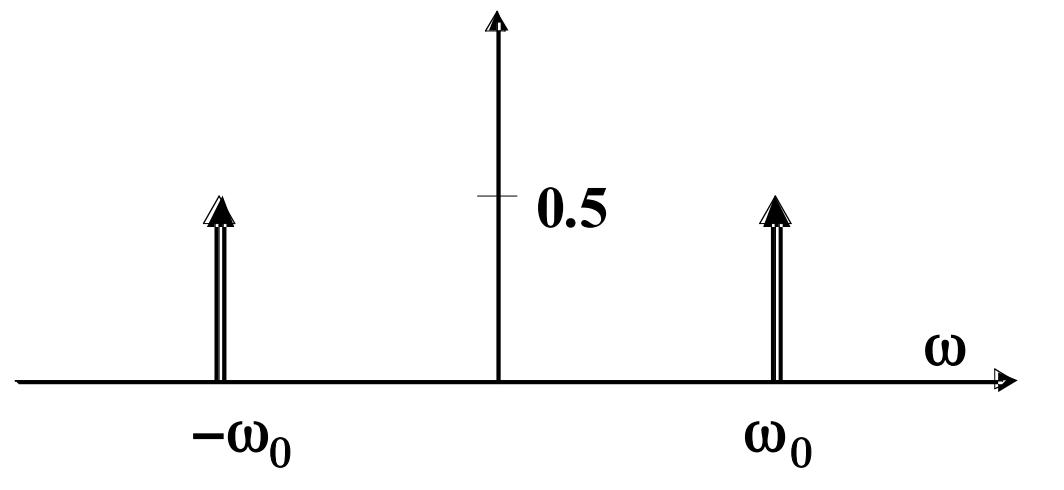
\includegraphics[width=4.5cm]{sin-mod} \caption{}
			\end{subfigure}
			\begin{subfigure}{0.48\linewidth}
				\centering
				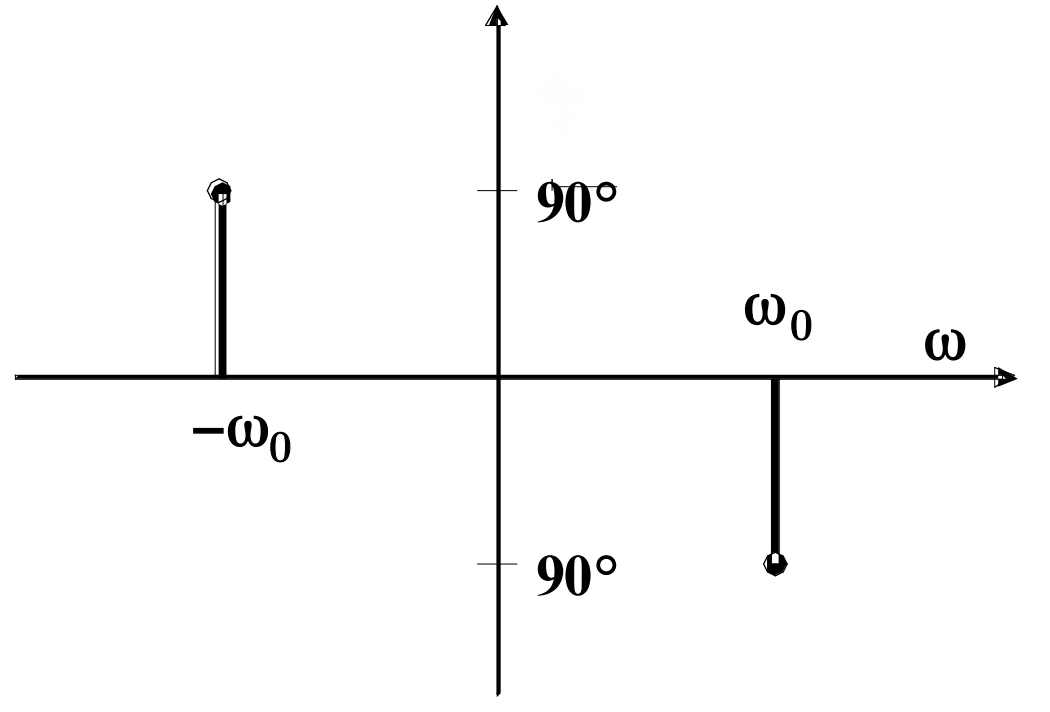
\includegraphics[width=4.5cm]{sin-ang} \caption{}
			\end{subfigure}
			\caption{modulo (a) e fase (b) dello spettro della funzione $\sin(\omega_0 t)$.}
			\label{fig:four:spettroseno}
		\end{figure}
		
		Per via della definizione della funzione $\delta$ di Dirac, scelta una qualsiasi funzione di trasferimento $H(\omega)$ risulta verificato che l'integrale in tutto lo spettro delle frequenze coincide di fatto con il valore della pulsazione della funzione $H(\omega)$ valutata nell'istante $\omega_0$ nel quale avviene l'impulso:
		\[ \int_{-\infty}^\infty H(\omega)\, \delta(\omega-\omega_0) \, d\omega = H(\omega_0)\]
		\begin{nota}
			La funzione $\delta$ moltiplica per un valore infinito il valore di $H$ nel punto $\omega_0$ (annullando il resto del dominio), tuttavia integrando in un intervallo infinitesimo $d\omega$ dello stesso ordine dell'infinito, i due termini si \textit{elidono} portando al risultato mostrato.
		\end{nota}
		
		Scomponendo la funzione di trasferimento $H$ nel suo modulo $M$ e fase $\phi$ secondo la relazione $H(\omega) = M(\omega) e^{i\phi(\omega)}$ (dove $M(\omega)$ è sempre un valore scalare!)  è possibile calcolare la risposta del sistema attraverso il prodotto della funzione di trasferimento per lo spettro del segnale sinusoidale ricavato in precedenza, arrivando al risultato
		\begin{align*}
			Y(\omega) & = H(\omega) \, U(\omega) = H(\omega) \left(\frac i 2 \delta(\omega + \omega_0) - \frac i 2 \delta(\omega-\omega_0)\right) \\
			& = H(-\omega_0) \frac i 2 \delta(\omega+\omega_0) - H(\omega_0) \frac i 2 \delta(\omega-\omega_0) \\
			& = M(\omega_0) \frac i 2 \delta(\omega+\omega_0) e^{-i\phi(\omega_0)} - M(\omega_0) \frac i 2 \delta(\omega-\omega_0) e^{i\phi(\omega_0)}
		\end{align*}
		
		Considerando le proprietà dello spettro di un segnale che permettono di affermare che il modulo $M$ è simmetrico rispetto all'asse delle ordinate, mentre la fase $\phi$ è antisimmetrica, tramite manipolazione dell'equazione di Eulero $e^{i\phi} = \cos \phi + i\sin\phi$ è possibile esprimere il rapporto tra risposta $Y$ e modulo $M$ (valutato nella pulsazione del segnale originario) come
		\begin{equation*}
			\frac{Y(\omega)}{M(\omega_0)} = \cos \big(\phi(\omega_0)\big) \underbrace{\left[ \frac i 2 \delta(\omega+\omega_0) - \frac i 2 \delta(\omega-\omega_0)\right]}_{\four{\sin(\omega_0 t)}} + \sin \big(\phi(\omega_0)\big) \underbrace{\left[ \frac 1 2 \delta(\omega+\omega_0) + \frac 1 2 \delta(\omega-\omega_0)\right]}_{\four{\cos(\omega_0 t)}}
		\end{equation*}
		
		Osservando il risultato è possibile osservare che il coefficiente di $\cos\big(\phi(\omega_0)\big)$ coincide con la trasformata della funzione iniziale $\sin(\omega_0t)$, mentre è possibile dimostrare per analogia che il coefficiente di $\sin\big(\phi(\omega_0)\big)$ è pari alla trasformata del segnale cosinusoidale di pulsazione $\omega_0$:
		\[ \cos(\omega_0 t) \quad \mapsto \quad \frac 1 2 \delta(\omega+\omega_0) + \frac 1 2 \delta(\omega-\omega_0)  \]
		Condensando i risultati ottenuti è dunque possibile antitrasformare per ottenere la risposta del sistema nel dominio del tempo con il risultato che
		\begin{equation}
		\begin{split}
			y(t) & = M(\omega_0) \cos\big(\phi(\omega_0)\big) \sin(\omega_0t) + M(\omega_0) \sin\big(\phi(\omega_0)\big) \cos(\omega_0 t) \\
			& =M(\omega_0) \sin\big(\omega_0 t + \phi(\omega_0)\big)
		\end{split}
		\end{equation}
		
		Questa relazione ci permette dunque di capire che se un sistema di equazioni differenziali lineari presenta come ingresso forzante un ingresso armonico unitario di pulsazione $\omega_0$, allora l'uscita del sistema sarà un'altra armonica di pulsazione invariata $\omega_0$ che risulterà moltiplicato e sfasato in base alle componenti della funzione di trasferimento $H$ valutata nella pulsazione $\omega_0$; un altro modo per osservare che i moduli delle funzioni $H,U$ si moltiplicano mentre le fasi si sommano si poteva ricavare considerando che
		\[Y(\omega) = H(\omega) U(\omega) = M_H(\omega) e^{i\phi_H(\omega)} + M_U(\omega) e^{i\phi_U(\omega)} = M_H(\omega)M_U(\omega) e^{i \left( \phi_H(\omega) + \phi_U(\omega) \right)}\]
	
	\subsection{\textit{Discrete Fourier Transform}}
		Nella pratica di misura attualmente si effettua un'elaborazione di segnali digitali che sono dunque discretizzati nel tempo; il segnale in ingresso al sistema di misura non sarà più dunque una funzione continua nel tempo $s(t)$, ma potrà essere considerato come una sequenza di valori $s_k$; il tempo che intercorre tra un campione e l'altro è pari al \de{periodo di campionamento} $T_c$ che coincide con l'inverso della \de{frequenza di campionamento} $f_c$.
		
		Per analizzare questo tipo di segnali si ricorre alla \de{trasformata di Fourier discreta} \textbf{DFT} (\textit{Discrete Fourier Transform}), l'analogo della trasformata di Fourier per segnali discretizzati nel tempo e che si basa anch'essa sulla scomposizione in basi ortonormali. L'algoritmo  che si occupa di trasformare segnali discreti prende il nome di \textbf{FFT} \de{\textit{Fast Fourier Transform}}.
		
		Data dunque una serie di $n$ di campioni $s_i$ discretizzati, la sequenza $Sf_n$ ottenuta dalla DFT sarà composta da un numero di elementi pari a $n$ (numero di campioni analizzati) con una risoluzione in frequenza pari a 
		\[ \Delta_f = \frac 1 {n\,T_c}\]
		La risoluzione in frequenza si può ottenere considerando che alla frequenza di campionamento $f_c$ il periodo temporale che intercorre per analizzare $n$ campioni è proprio pari a $n T_c$ e dunque la minima frequenza presente nel segnale è pari all'inverso di tale valore.
		
		In realtà per il \textbf{teorema di Nyquist} è possibile osservare che dello spettro ricavato, solo la prima meta (associato alle frequenze inferiori a $f_c/2$) ha un significato reale, in quanto i successivi valori ottenuti sono la copia ribaltata della prima parte dello spettro (dovuto alla simmetria delle componenti negative). Il valore $f_n = f_c/2$ prende dunque il nome di \de{frequenza di Nyquist} e rappresenta la frequenza limite dello spettro che si può ricavare dalla DFT.
		
		\figura{6}{1}{dft-simmetria}{esempio di DFT di un segnale; è possibile osservare la specularità dello spettro rispetto al punto medio.}{dft-simmetria}
		
		
\section{Taratura dinamica}
	\marginnote{27/04/2021}
	
	Durante la taratura statica si effettua la stima dei coefficienti di una relazione matematica (tendenzialmente polinomiale) che lega il misurando con l'uscita dello strumento in condizioni statiche. Dualmente si effettua una \de{taratura dinamica} quando si vuole stimare i coefficienti delle relazioni che governano la dinamica tra misurando e uscita dello strumento. Questo problema è strettamente legato alla risoluzione di equazioni differenziali e, ipotizzando che le stesse siano lineari, è possibile dunque risolvere il problema utilizzandola trasformata di Fourier.
	
	La taratura dinamica si occupa di determinare i parametri della funzione complessa di trasferimento $H(\omega)$ del sistema di misura nel caso in cui:
	\begin{itemize}
		\item non si conosce il modello matematico ne i parametri del sistema di misura. In questo caso è necessario determinare la funzione di trasferimento direttamente nel dominio della frequenza in quanto nessuna informazione è nota a priori;
		\item il modello matematico è noto, ma non i suoi parametri. In questo caso conoscendo l'equazione differenziale che regola la relazione ingresso-uscita è sufficiente stimare i parametri mediante delle tecniche nel dominio del tempo.
	\end{itemize}
	
	\subsection{Tecniche nel dominio della frequenza}

	Per effettuare la taratura è possibile imporre degli \textbf{ingressi armonici} variabili in ingresso; noto infatti l'ingresso $u(t) = \sin(\omega_0 t)$, allora l'uscita del sistema (per quanto visto dall'analisi di Fourier) dipende dalla funzione di trasferimento nel punto $\omega_0$ definita come $H(\omega_0) = M(\omega_0) e^{i\phi(\omega_0)}$ secondo la legge
	\[ y(t) = M(\omega_0 ) \sin \big(\omega_0 t+ \phi(\omega_0) \big)\]
	
	Variando il parametro $\omega_0$ è possibile misurare sia i coefficienti $M(\omega)$, sia gli sfasamenti $\phi(\omega)$ e dunque per interpolazione è possibile ricavare il modello del sistema dinamico.
	
	Per generare i segnali sinusoidali armonici per sistemi meccanici si utilizza un cosiddetto \textit{shaker} (una forza sinusoidale può essere trasmessa da una barra magnetica immersa in un solenoide che, con una corrente alternata, impone un momento, e dunque una forza, sinusoidale), mentre per componenti elettrici è possibile costruire degli opportuni sistemi. Per sistemi di misura termici  non è possibile generare degli ingressi sinusoidali.
	
	\begin{nota}
		In generale non tutti i sistemi da tarare possono essere analizzati imponento un ingresso sinusoidale di frequenza nota.	
	\end{nota}
	
	Un altro modo per analizzare la funzione di trasferimento è quello di analizzare la risposta all'impulso del sistema in quanto essa rappresenta l'antitrasformata della funzione di trasferimento (per quanto visto in precedenza). Imponendo dunque un impulso e trasformando il segnale temporale conseguente nel dominio della frequenza si ottiene la funzione di trasferimento.
	
	\vspace{3mm}
	\textbf{DA RIVEDERE UN PO LA DESCRIZIONE DI QUESTA PARTE}
	
	Supponendo invece di porre in ingresso un valore costante allora è possibile verificare che
	\[ Y(\omega) = M_H( \omega) e^{i\phi_H(\omega)} \cancel{M_U(\omega)} e^{i\phi_U(\omega)} = M_H(\omega) e^{i \left[ \phi_H(\omega) + \phi_U(\omega) \right]}  \qquad \Rightarrow M_H(\omega) =M_Y(\omega)	\]
	\textit{Si usano segnali qualsiasi per avere la certezza che $U\neq0$ per ogni frequenza $\omega$ in modo da non avere buchi nello spettro.}
	
	
	
	\paragraph{Modello noto} Considerando di conoscere il modello dello strumento, per effettuare la taratura dinamica è possibile utilizzare degli ingressi canonici effettuando la taratura minimizzando gli scarti quadratici medi.
	
	Considerando per esempio una sonda \texttt{PT100} per la misura della temperatura realizzata da un filo trasduttore in platino, è possibile calcolare l'energia $E$ dello strumento posto a temperatura assoluta $T$ e il flusso di calore tra sonda e ambiente $P$ come
	\[E=mc T \qquad P = \alpha A \big(T_{amb} - T\big) \]
	Il modello matematico del problema è dato dall'equazione differenziale
	\[ \frac{dE}{dt} = P \qquad \rightarrow \quad mc \frac {dT}{dt} = \alpha A \big(T_{amb} - T \big)  \]
	Trasformando questa equazione nel dominio della frequenza tramite Fourier si ricava che
	\[ u\omega m c = \alpha A \big(T_{amb}(\omega) \omega -T(\omega)\big) \qquad T(\omega) \big(i\omega m c + \alpha a\big) = \alpha A T_{amb}(\omega)\]
	Dovendo misurare la temperatura $T_{amb}$ valutando la temperatura $T$ è possibile connotare la funzione di trasferimento come
	\[ H(\omega) = \frac 1 {1 + i\omega \frac{mc}{\alpha A}}\]
	dove $\frac{mc}{\alpha A} = \tau$ è l'unico parametro temporale del sistema che deve essere valutato tramite la taratura dinamica.
	
	Per la taratura si impone un ingresso a scalino inserendo la sonda (che stava libera all'aria) velocemente in un contenitore pieno di fluido caldo/freddo. L'inserimento che può richiedere $1/10s$ (e dunque $10Hz$) può essere considerato istantaneo se si misura che la costante di tempo $\tau$ del sistema di misura risulta valere $50s$(e dunque $0.02Hz \ll 10Hz$).
	
	Nel dominio del tempo è possibile calcolare la temperatura $T(t)$ misurata come
	\[T(t) = \big(T_{iniz} - T_{fin}\big) e^{-t/\tau} + T_{fin} \]
	Per ricavare il parametro $\tau$ del sistema è possibile ricorrere a più metodi:
	\begin{enumerate}
		\item il primo è basato sulla manipolazione dell'equazione algebrica che risolve l'equazione differenziale per l'ingresso allo scalino, in particolare si trovando la temperatura $T(\tau)$ associata al tempo $t=\tau$ si determina il valore della costante:
		\[ T(\tau) = \big(T_{iniz} - T_{fin}\big) e^{-1} + T_{fin} \]
		
		\item \textit{riscalo temperatura per renderla lineare}
	\end{enumerate}

	\paragraph{Filtraggio online e offline} Si parla di \textbf{filtraggio online} quando l'operazione di filtraggio viene effettuata ad ogni campione in ingresso (\textit{processing in real time}), mentre si parla di \textbf{filtraggio offline} quando il filtraggio viene effettuato sull'insieme di dati già acquisiti.
	
	Un filtro online discreto semplice è quello del primo ordine per il quale un ingresso $u(t)$ (e dunque $U(\omega)$) viene modificato in un'uscita $y(t)$ (analogamente $Y(\omega)$) da un fattore moltiplicativo
	\[ \frac 1 {1 + i\omega \tau} \qquad \xrightarrow{Y(\omega) = G U(\omega)} Y(\omega) + \tau i \omega Y(\omega) = U(\omega) \]
	Antitrasformando con Fourier questa relazione si ricava l'equazione differenziale che governa l'uscita
	\[y(t) + \tau \frac{dy(t)}{dt} = u(t)\]
	Discretizzando questa equazione continua (utilizzando la derivata di Eulero come approssimazione di $dy/dt$) si ottiene la funzione discretizzata
	\[ y_k + \tau \frac{y_k - y_{k-1}}{T_c} = y_k \left(1 + \frac \tau {T_c} \right) - \frac \tau {T_c} y_{k-1} = u_{k-1} \]
	\[  \Rightarrow \quad y_k = \frac{\tau / T_c}{1 + \frac{\tau}{T_c}} y_{k-1} + \frac 1  { 1+ \frac \tau {T_c}} u_{k-1} \]
	Questa successione per ricorrenza permette di capire coma lavora un filtro digitale, ossia i coefficienti $a$ e $b$ da porre prima dei valori $y_{k-1}$ e $u_{k-1}$ per calcolare $y_k$. Il problema di questo tipo di filtri è che introducono un ritardo nella misura.
	
	Uno strumento di misura dinamica ideale è quello con frequenza di taglio di molto maggiore della frequenza caratteristica del problema in quanto lascia invariato il modulo della risposta in frequenza e non introduce alcun sfasamento, tuttavia questo non sempre è possibile. Un modo per ridurre questo problema sarebbe di filtrare il segnale in uscita con un filtro inverso $H^{-1}$ che permette, teoricamente, di ripristrinare il segnale originario. Tuttavia questo metodologia non annullerebbe il rumore bianco che tenderebbe ad \textit{esplodere}. 
	
	\vspace{3mm}
	Un filtraggio offline invece non introduce degli sfasamenti ma, avendo un'istantanea di tutto il segnale campionato, è possibile attenuare delle frequenze determinate senza cambiarne la fase.
	
	
	
	
	
	\begin{esempio}{: taratura di una sonda termica}
		Si consideri una sonda \texttt{PT-100} composta da un filamento in platino posto ad una temperatura $T_s$ con massa $m_s$ e capacità termica $c_s$; la sonda è rivestita da una guaina di temperatura $T_g$, massa $m_g$ e capacità $c_g$ e lo scambio termico di coefficiente $\alpha_{gs}$ avviene tra un'area di contatto $A_{gs}$. La guaina è immessa in un un fluido a temperatura $T_m$ e la superficie di contatto pari a $A_{mg}$ con coefficiente $\alpha_{mg}$.
		
		Le equazioni differenziali che governano il problema sono dunque
		\[ m_s c_s \frac{dT_s}{dt} \alpha_{gs} A_{gs} \big(T_g -T_s\big) \qquad m_g c_g \frac{dT_g}{dt} = \alpha_{mg} A_{mg} \big(T_m-T_g\big) + \alpha_{gs}A_{gs}(T_s- T_g)\]
		
		Per calcolare la funzione di trasferimento del sistema è necessario trasformare le equazioni nel dominio delle frequenze; considerando la prima equazione si ottiene l'espressione
		\[m_s c_s i\omega T_s(\omega) = \alpha_{gs} A_{gs}\Big( T_{g}(\omega) - T_{s}(\omega)\Big) \]
		dalla quale si ricava la temperatura $T_g$ in funzione della temperatura $T_s$:
		\[ T_g(\omega) = T_s(\omega) \frac{m_s c_s i\omega + \alpha_{gs} A_{gs}}{\alpha_{gs}A_{gs}} \]
		
		Trasformando la seconda equazione differenziale nel dominio della frequenza e sostituendo il valore di $T_g$ come appena determinato è possibile determinare
		\[ m_g c_g i\omega T_g(\omega) = \alpha_{mg} A_{mg} \Big(T_m(\omega) - T_g(\omega)\Big) + \alpha_{gs} A_{gs} \Big(T_s(\omega) - T_g(\omega)\Big) \]
		\[ \Rightarrow \quad H(\omega) = \frac 1 {1 + i\omega \dfrac{m_s c_s (\alpha_{mg} A_{mg} + \alpha_{gs} A_{gs} ) + m_g c_g \alpha_{gs} A_{gs} }{\alpha_{gs} A_{gs}\alpha_{mg} A_{mg} }  + \big(i\omega\big)^2 \dfrac{m_s c_s m_g c_g}{\alpha_{gs} A_{gs} \alpha_{mg} A_{mg} } } \]
		
		Si osserva dunque che la funzione di trasferimento è del secondo ordine in quanto a denominatore contiene un termine $\omega^2$.
		
	\end{esempio}
	
	
	
	
	
	
	
	
	
	
	
	
	
	
	
	
	
	
	
	
	
	
	